%
% 						Main document Project Zephyr
% ===========================================================================


%---------------------------------------------------------------------------
\documentclass[
	a4paper,												% paper format
	10pt,													% fontsize
	twoside,												% double-sided
	openright,												% begin new chapter on right side
	notitlepage,											% use no standard title page
	parskip=half,											% set paragraph skip to half of a line
]{scrreprt}
%---------------------------------------------------------------------------

\raggedbottom
\KOMAoptions{cleardoublepage=plain}							% Add header and footer on blank pages


% Load Standard Packages:
%---------------------------------------------------------------------------
\usepackage[standard-baselineskips]{cmbright}

\usepackage[ngerman]{babel}									% german hyphenation
%\usepackage[latin1]{inputenc}  							% Unix/Linux - load extended character set (ISO 8859-1)
\usepackage[ansinew]{inputenc}  							% Windows - load extended character set (ISO 8859-1)
\usepackage[T1]{fontenc}									% hyphenation of words with ä,ö and ü
\usepackage{textcomp}										% additional symbols
\usepackage{ae}												% better resolution of Type1-Fonts 
\usepackage{fancyhdr}										% simple manipulation of header and footer 
\usepackage{etoolbox}										% color manipulation of header and footer
\usepackage{graphicx}                      					% integration of images
\usepackage{float}											% floating objects
\usepackage{caption}										% for captions of figureMain documents and tables
\usepackage{booktabs}										% package for nicer tables
\usepackage{tocvsec2}										% provides means of controlling the sectional numbering
%---------------------------------------------------------------------------

% Load Math Packages
%---------------------------------------------------------------------------
\usepackage{amsmath}                    	   				% various features to facilitate writing math formulas
\usepackage{amsthm}                       	 				% enhanced version of latex's newtheorem
\usepackage{amsfonts}                      					% set of miscellaneous TeX fonts that augment the standard CM
\usepackage{amssymb}										% mathematical special characters
\usepackage{exscale}										% mathematical size corresponds to textsize
%---------------------------------------------------------------------------

% Package to facilitate placement of boxes at absolute positions
%---------------------------------------------------------------------------
\usepackage[absolute]{textpos}
\setlength{\TPHorizModule}{1mm}
\setlength{\TPVertModule}{1mm}
%---------------------------------------------------------------------------					
			
% Definition of Colors
%---------------------------------------------------------------------------
\RequirePackage{color}                         				% Color (not xcolor!)
\definecolor{linkblue}{rgb}{0,0,0.8}            			% Standard
\definecolor{darkblue}{rgb}{0,0.08,0.45}        			% Dark blue
\definecolor{bfhgrey}{rgb}{0.41,0.49,0.57}     	 			%  BFH grey
%\definecolor{linkcolor}{rgb}{0,0,0.8}     					% Blue for the web- and cd-version!
\definecolor{linkcolor}{rgb}{0,0,0}        					% Black for the print-version!
%---------------------------------------------------------------------------

% Hyperref Package (Create links in a pdf)
%---------------------------------------------------------------------------
\usepackage[
	pdftex,ngerman,bookmarks,plainpages=false,pdfpagelabels,
	backref = {false},										% No index backreference
	colorlinks = {true},                  					% Color links in a PDF
	hypertexnames = {true},              					% no failures "same page(i)"
	bookmarksopen = {true},               					% opens the bar on the left side
	bookmarksopenlevel = {0},             					% depth of opened bookmarks
	pdftitle = {Template fuer Bachelor Thesis},	 			%  PDF-property
	pdfauthor = {brd3},        					 			%  PDF-property
	pdfsubject = {LaTeX Template},        					%  PDF-property
	linkcolor = {linkcolor},              					% Color of Links
	citecolor = {linkcolor},              					% Color of Cite-Links
	urlcolor = {linkcolor},               					% Color of URLs
]{hyperref}
%---------------------------------------------------------------------------

% Set up page dimension
%---------------------------------------------------------------------------
\usepackage{geometry}
\geometry{
	a4paper,
	left=28mm,
	right=15mm,
	top=30mm,
	headheight=20mm,
	headsep=10mm,
	textheight=242mm,
	footskip=15mm
}
%---------------------------------------------------------------------------

% Makeindex Package
%---------------------------------------------------------------------------
\usepackage{makeidx}                         				% To produce index
\makeindex                                    				% Index-Initialisation
%---------------------------------------------------------------------------

% Glossary Package
%---------------------------------------------------------------------------
% the glossaries package uses makeindex
% if you use TeXnicCenter do the following steps:
%  - Goto "Ausgabeprofile definieren" (ctrl + F7)
%  - Select the profile "LaTeX => PDF"
%  - Add in register "Nachbearbeitung" a new "Postprozessoren" point named Glossar
%  - Select makeindex.exe in the field "Anwendung" ( ..\MiKTeX x.x\miktex\bin\makeindex.exe )
%  - Add this [ -s "%tm.ist" -t "%tm.glg" -o "%tm.gls" "%tm.glo" ] in the field "Argumente"
%
% for futher informations go to http://ewus.de/tipp-1029.html
%---------------------------------------------------------------------------
\usepackage[nonumberlist]{glossaries}
\makeglossaries

\newglossaryentry{BibTeX}{name={BibTeX},description={Programm zur Erstellung von Literaturangaben und -verzeichnissen in \TeX- oder \LaTeX-Dokumenten}}
\newglossaryentry{StwVrz}{name={Stichwortverzeichnis},description={Verzeichnis mit Stichworten aus dem Text}}



%---------------------------------------------------------------------------

% Intro:
%---------------------------------------------------------------------------
\begin{document}                              				% Start Document
\settocdepth{section}										% Set depth of toc
\pagenumbering{roman}														
%---------------------------------------------------------------------------

\providecommand{\titel}{Zephyr-Projekt}		% Titel der Projektarbeit										% Titel der Arbeit aus Datei titel.tex lesen
\providecommand{\versionnumber}{0.1}			%  Aktuelle Versionsnummer eingeben
\providecommand{\versiondate}{29.09.2016}		%  Datum der aktuellen Version eingeben									% Versionsnummer und -datum aus Datei version.tex lesen

% Set up header and footer
%---------------------------------------------------------------------------
\makeatletter
\patchcmd{\@fancyhead}{\rlap}{\color{bfhgrey}\rlap}{}{}		% new color of header
\patchcmd{\@fancyfoot}{\rlap}{\color{bfhgrey}\rlap}{}{}		% new color of footer
\makeatother

\fancyhf{}													% clean all fields
\fancypagestyle{plain}{										% new definition of plain style	
	\fancyfoot[OR,EL]{\footnotesize \thepage} 				% footer right part --> page number
	\fancyfoot[OL,ER]{\footnotesize \titel, Version \versionnumber, \versiondate}	% footer even page left part 
}

\renewcommand{\chaptermark}[1]{\markboth{\thechapter.  #1}{}}
\renewcommand{\headrulewidth}{0pt}							% no header stripline
\renewcommand{\footrulewidth}{0pt} 							% no bottom stripline

\pagestyle{plain}
%---------------------------------------------------------------------------


% Title Page and Abstract
%---------------------------------------------------------------------------
%%
% Project documentation template
% ===========================================================================
% This is part of the document "Project documentation template".
% Authors: brd3, kaa1
%

\begin{titlepage}


% BFH-Logo absolute placed at (28,12) on A4 
% Actually not a realy satisfactory solution but working.
%---------------------------------------------------------------------------
\setlength{\unitlength}{1mm}
\begin{textblock}{20}[0,0](28,12)
	
\includegraphics[scale=1.0]{bilder/BFH_Logo_B.png}
\end{textblock}
\color{black}

% Institution / Titel / Untertitel / Autoren / Experten:
%---------------------------------------------------------------------------
\begin{flushleft}

\vspace*{21mm}

\fontsize{26pt}{40pt}\selectfont 
\titel 				\\							% Titel aus der Datei vorspann/titel.tex lesen
\vspace{2mm}

\fontsize{16pt}{24pt}\selectfont\vspace{0.3em}
Hier steht ein Untertitel 			\\							% Untertitel eingeben
\vspace{5mm}

\fontsize{10pt}{12pt}\selectfont
\textbf{Art der Arbeit (Semesterarbeit / Bachelorthesis / etc.)} \\									% eingeben
\vspace{7mm}

% Abstract (eingeben):
%---------------------------------------------------------------------------
\begin{textblock}{150}(28,100)
\fontsize{10pt}{12pt}\selectfont
[Kurztext (Abstract) einf�gen, falls gew�nscht] \\ 
Dieses Dokument dient als Vorlage f�r die Erstellung von Berichten nach den Richtlinien der BFH. Die Vorlage ist in \LaTeX{} erstellt und unterst�tzt das automatische Erstellen von diversen Verzeichnissen, Literaturangaben, Indexierung und Glossaren. Dieser kleine Text ist eine Zusammenfassung �ber das vorliegenden Dokument mit einer L�nge von 4 bis max. 8 Zeilen. \\
Das Titelbild kann in den Zeilen 157/158 der Datei template.tex ein- oder ausgeschaltet werden.
\end{textblock}

\begin{textblock}{150}(28,225)
\fontsize{10pt}{17pt}\selectfont
\begin{tabbing}
xxxxxxxxxxxxxxx\=xxxxxxxxxxxxxxxxxxxxxxxxxxxxxxxxxxxxxxxxxxxxxxx \kill
Studiengang:	\> [z.B. Elektro- und Kommunikationstechnik]	\\			% Namen eingeben
Autoren:		\> [Test Peter, M�ster R�s�]		\\					% Namen eingeben
Betreuer:	\> [Dr.~Xxxx Xxxx, Dr.~Yyyy Yyyy]		\\					% Namen eingeben
Auftraggeber:	\> [Wwwww AG]						\\					% Namen eingeben
Experten:		\> [Dr.~Zzzz Zzzz]				\\					% Namen eingeben
Datum:			\> \versiondate					\\		% aus Datei vorspann/version.tex lesen
\end{tabbing}

\end{textblock}
\end{flushleft}

\begin{textblock}{150}(28,280)
\noindent 
\color{bfhgrey}\fontsize{9pt}{10pt}\selectfont
Berner Fachhochschule | Haute �cole sp�cialis�e bernoise | Bern University of Applied Sciences
\color{black}\selectfont
\end{textblock}


\end{titlepage}

%
% ===========================================================================
% EOF
%
					% activate for Titelseite ohne Bild
%
% Project documentation template
% ===========================================================================


\begin{titlepage}


% BFH-Logo absolute placed at (28,12) on A4 and picture (16:9 or 15cm x 8.5cm)
% Actually not a realy satisfactory solution but working.
%---------------------------------------------------------------------------
\setlength{\unitlength}{1mm}
\begin{textblock}{20}[0,0](28,12)
	
\includegraphics[scale=1.0]{bilder/BFH_Logo_B.png}
\end{textblock}

\begin{textblock}{154}(28,48)
	\begin{picture}(150,2)
		\put(0,0){\color{bfhgrey}\rule{150mm}{2mm}}
	\end{picture}
\end{textblock}

\begin{textblock}{154}[0,0](28,50)
	
\includegraphics[scale=1.0]{bilder/Zephyr-Project.jpg}			% Titelbild definieren
\end{textblock}

\begin{textblock}{154}(28,135)
	\begin{picture}(150,2)
		\put(0,0){\color{bfhgrey}\rule{150mm}{2mm}}
	\end{picture}
\end{textblock}
\color{black}

% Institution / Titel / Untertitel / Autoren / Experten:
%---------------------------------------------------------------------------
\begin{flushleft}

\vspace*{115mm}

\fontsize{26pt}{28pt}\selectfont 
\titel 				\\							% Titel aus der Datei vorspann/titel.tex lesen
\vspace{2mm}

\fontsize{16pt}{20pt}\selectfont\vspace{0.3em}
Echtzeit-OS f�r das Internet der Dinge 			\\							% Untertitel eingeben
\vspace{5mm}

\fontsize{10pt}{12pt}\selectfont
\textbf{Projektarbeit} \\									% eingeben
\vspace{3mm}

% Abstract (eingeben):
%---------------------------------------------------------------------------
\begin{textblock}{150}(28,190)
\fontsize{10pt}{12pt}\selectfont
Die Linux Foundation hat mit dem Projekt Zephyr mit der Entwicklung eines Echtzeit-Betriebssystems f�r das Internet der Dinge (IoT) begonnen.
Zephyr ist ein Open-Source-Betriebssystem mit dem Ziel ein solides OS f�r IoT Ger�te mit geringen Ressourcen bereitzustellen. Es nutzt eine echtzeitf�hige Kombination aus Nano- und Microkernel. 
Im Gegensatz zu einem Linux Kernel ben�tigt Zephyr nur zwischen 8 und 512 KByte an Arbeitsspeicher.  Aktuell werden folgenden Plattformen unterst�tzt: x86, ARM und ARC EM4
\end{textblock}

\begin{textblock}{150}(28,225)
\fontsize{10pt}{17pt}\selectfont
\begin{tabbing}
xxxxxxxxxxxxxxx\=xxxxxxxxxxxxxxxxxxxxxxxxxxxxxxxxxxxxxxxxxxxxxxx \kill
Studiengang:	\> Elektro- und Kommunikationstechnik			\\
Autoren:		\> Aaron Schmocker, David Wyss					\\
Betreuer:		\> Martin Aebersold								\\
Auftraggeber:	\> Martin Aebersold								\\
Experten:		\> Martin Aebersold								\\
Datum:			\> \versiondate									\\
\end{tabbing}

\end{textblock}
\end{flushleft}

\begin{textblock}{150}(28,280)
\noindent 
\color{bfhgrey}\fontsize{9pt}{10pt}\selectfont
Berner Fachhochschule | Haute �cole sp�cialis�e bernoise | Bern University of Applied Sciences
\color{black}\selectfont
\end{textblock}


\end{titlepage}

%
% ===========================================================================
% EOF
%
						% activate for Titelseite mit Bild
% Versionenkontrolle :
% -----------------------------------------------

\begin{textblock}{180}(15,150)
\color{black}
\begin{huge}
Versionen
\end{huge}
\vspace{10mm}

\fontsize{10pt}{18pt}\selectfont
\begin{tabbing}
xxxxxxxxxxx\=xxxxxxxxxxxxxxx\=xxxxxxxxxxxxxx\=xxxxxxxxxxxxxxxxxxxxxxxxxxxxxxxxxxxxxxxxxxxxxxx \kill
Version	\> Datum	\> Status		\> Bemerkungen \\
0.1	\> 29.09.2016	\> Entwurf		\> Titelblatt erstellt und Template f�r Linux angepasst \\	
%0.2	\> 21.08.2016	\> Entwurf		\> Phasellus scelerisque \\ 
%0.3	\> 02.09.2016	\> Entwurf		\> Donec eget aliquam urna. Lorem ipsum dolor sit amet \\ 
%1.0	\> 12.09.2016	\> Definitiv	\> Lorem ipsum dolor sit ametPhasellus scelerisque, leo sed iaculis ornare \\ 
%1.1	\> 04.11.2016	\> Korrektur	\> Layout angepasst \\
%1.2	\> 01.02.2016	\> Erg�nzung	\> Kapitel 1.1 erweitert \\
\end{tabbing}

\end{textblock}

\cleardoubleemptypage
\setcounter{page}{1}
\cleardoublepage
\phantomsection 
\addcontentsline{toc}{chapter}{Management Summary}
\chapter*{Management Summary}
\label{chap:managementSummary}

Lorem ipsum dolor sit amet, consectetur adipiscing elit. Phasellus scelerisque, leo sed iaculis ornare, mi leo semper urna, ac elementum libero est at risus. Donec eget aliquam urna. Lorem ipsum dolor sit amet, consectetur adipiscing elit. Nunc fermentum nunc sollicitudin leo porttitor volutpat. Duis ac enim lectus, quis malesuada lectus. Aenean vestibulum suscipit justo, in suscipit augue venenatis a. Donec interdum nibh ligula. Aliquam vitae dui a odio cursus interdum quis vitae mi. Phasellus ornare tortor fringilla velit accumsan quis tincidunt magna eleifend. Praesent nisl nibh, cursus in mattis ac, ultrices ac nulla. Nulla ante urna, aliquet eu tempus ut, feugiat id nisl. Nunc sit amet mauris vitae turpis scelerisque mattis et sed metus. Aliquam interdum congue odio, sed semper elit ullamcorper vitae. Morbi orci elit, feugiat vel hendrerit nec, sollicitudin non massa. Quisque lacus metus, vulputate id ullamcorper id, consequat eget orci \nocite{kopka:band1} \nocite{Marti06}. 

\cleardoubleemptypage
%---------------------------------------------------------------------------

% Table of contents
%---------------------------------------------------------------------------
\tableofcontents
\cleardoublepage
%---------------------------------------------------------------------------

% Main part:
%---------------------------------------------------------------------------
\pagenumbering{arabic}

\chapter{Einleitung}
\label{chap:einleitung}

Dieses Dokument dient einerseites zur Illustration der \LaTeX{} Vorlage anhand des Corporate Designs\index{Corporate Design} der Berner Fachhochschule\index{Berner Fachhochschule} und andererseits als Anleitung f�r deren Verwendung. Dabei wird vorausgesetzt, dass der Benutzer bereits Erfahrungen mit \LaTeX{} besitzt oder gewillt ist, sich w�hrend der Benutzung in das Thema einzuarbeiten. Im Quellenverzeichnis sind einige n�tzliche Eintr�ge zu diversen B�chern und Dokumenten im Internet �ber \LaTeX{} zu finden.

% Eintr�ge im Verzeichnis erscheinen lassen ohne hier eine Referenz einzuf�gen
\nocite{kopka:band1}
\nocite{raichle:bibtex_programmierung}
\nocite{MiKTeX}
\nocite{KOMA}
\nocite{TeXnicCenter}
\nocite{Marti06}
\nocite{Erbsland08}
\nocite{juergens:einfuehrung}
\nocite{juergens:fortgeschritten}

\section{Dokumentaufbau}
\label{sec:einleitung_aufbau}

Das vorliegende Dokument ist so aufgebaut wie die Dokumentation einer Projektarbeit oder Thesis\index{Thesis}. Im Kapitel \ref{chap:anleitungen} werden die verwendeten Pakete kurz erkl�rt und Hinweise gegeben, wie die Bibliographie und das Glossar zu verwenden sind. Kapitel \ref{chap:satzspiegeltest} stellt ein reines Beispielkapitel dar, um den Satzspiegel zu pr�fen.

In Abbildung \ref{fig:datei_struktur} ist die Dateistruktur dieses Template dargestellt.

\begin{figure}[H]
	\centering
		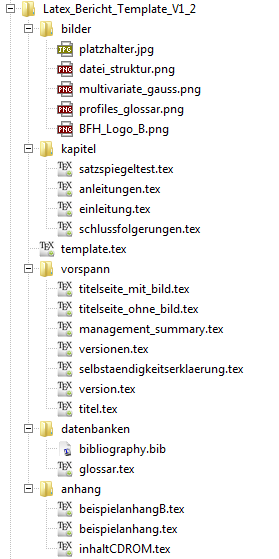
\includegraphics[scale=0.85]{bilder/datei_struktur.png}
	\caption{Dateistruktur}
	\label{fig:datei_struktur}
\end{figure}

\section{Kontakt}
\label{sec:einleitung_kontakt}

Die Hersteller dieser Vorlage sind nat�rlich froh um Verbesserungsvorschl�ge jeder Art. Kapitel \ref{sec:einleitung_vorschlaege} enth�lt m�gliche Verbesserungsvorschl�ge\index{Verbesserungsvorschl�ge}.

\begin{table}[H]
	\centering
		\begin{tabular}{lll} \toprule
			\textbf{Vorname Name} & \textbf{E-Mail} & \textbf{Funktion} \\ \midrule
			Alfred Kaufmann & alfred.kaufmann@bfh.ch & Auftraggeber, Projektleitung, Erg�nzungen \\ \midrule
			Fritz Dellsperger & in Pension & Tipps zur Struktur und Layout \\ \midrule
			David Burri & ausgetreten & Erstellung der Vorlage \\ \bottomrule
		\end{tabular}
	\caption{Kontaktpersonen}
	\label{tab:kontaktpersonen}
\end{table}


\section{Verbesserungsvorschl�ge}
\label{sec:einleitung_vorschlaege}

\begin{itemize}
	\item Erstellen eines eigenen BFH Style-Files
	\item Vorlage f�r die Pr�sentationserstellung mit \LaTeX{}
\end{itemize}



\chapter{Anleitungen}
\label{chap:anleitungen}

Die nachfolgende Tabelle zeigt einige der wichtigsten Pakete\index{Paket}, die in der \LaTeX{} Vorlage verwendet werden.

\begin{table}[H]
	\centering
		\begin{tabular}{p{0.13\textwidth} p{0.75\textwidth}} \toprule
			\textbf{Paket} & \textbf{Funktion} \\ \midrule
			\texttt{cmbright}\index{cmbright} & Serifenlose Schriftart 'Computer Modern Bright' welche die Textcodierungen\index{Textcodierungen} OT1, T1 und TS1 unterst�tzt, sowie die mathematischen Zeichen wie auch die AMS Symbole \\ \midrule
			\texttt{ae} & Sorgt f�r besser aufgel�ste Schriften in PDF Dateien \\ \midrule
			\texttt{fancyhdr}\index{fancyhdr} & Einfache Anpassung der Kopf- und Fusszeilen \\ \midrule
			\texttt{graphicx}\index{graphicx} & Einbindung von Grafiken in \LaTeX{} dokumente \\ \midrule
			\texttt{booktabs}\index{booktabs} & Sch�nere Darstellung von Tabellen \\ \midrule
			\texttt{textpos}\index{textpos} & Vereinfachte absolute Positionierung von Boxen auf der Seite \\ \midrule
			\texttt{hyperref}\index{hyperref} & Paket zum Erstellen von Links in PDF Dateien \\ \midrule
			\texttt{geometry}\index{geometry} & Vereinfachte und verbesserte Anpassung des Standard-Satzspiegels \\ \midrule
			\texttt{makeidx}\index{makeidx} & Einfache Indexerstellung (siehe Kapitel \ref{sec:anleitungen_index})\\ \midrule
			\texttt{glossaries}\index{glossaries} & Erstellen von Glossaren (siehe Kapitel \ref{sec:anleitungen_glossar}) \\ \bottomrule
		\end{tabular}
	\caption{Pakete}
	\label{tab:pakete}
\end{table}


\section{Stichwortverzeichnisse}
\label{sec:anleitungen_index}

\LaTeX{} ist in der Grundausstattung nicht f�hig ein \gls{StwVrz} \index{Stichwortverzeichnis} zu erstellen. Diese k�nnen in \LaTeX{} mit dem \texttt{makeidx} Paket und dem \texttt{makeindex}\index{makeindex} Programm erstellt werden. Die folgende Seite enth�lt eine ausf�hrliche Erkl�rung wie das Paket funktioniert und dessen Anwendung:

\begin{center}
	\url{http://de.wikibooks.org/wiki/LaTeX-W%C3%B6rterbuch:_makeindex}
\end{center}

Grob zusammengefasst sind f�r ein Stichwortverzeichnis folgenden Punkte n�tig:

\begin{itemize}
	\item Einbinden des Paketes \texttt{makeidx}
	\item Durch den \texttt{\textbackslash makeindex} Befehl die Erstellung initialisieren
	\item Im Text laufend W�rter indexieren mit dem Befehl \texttt{\textbackslash index\{\}}
	\item Beim ersten Durchlauf der Dokumenterstellung wird das Verzeichnis erstellt und die mit \texttt{\textbackslash index\{\}} markierten Begriffe in der \texttt{.idx}-Datei gespeichert
	\item Beim zweiten Durchlauf wird die \texttt{.idx}-Datei sortiert, formatiert und als \texttt{.ind}-Datei abgespeichert, wobei \LaTeX{} nun die \texttt{.ind}-Datei in das Dokument einf�gt
\end{itemize}

\section{Glossar}
\label{sec:anleitungen_glossar}

Ein Glossar\index{Glossar} kann in \LaTeX{} ebenfalls mit dem \texttt{makeindex} Programm und dem \texttt{glossaries} Paket erstellt werden. Die folgende Auflistung zeigt das Vorgehen um ein Glossar zu erzeugen:

\begin{itemize}
	\item Einbinden des \texttt{glossaries} Pakets
	\item Falls es als sinnvoll erachtet wird, kann eine eigene Datenbank mit Glossareintr�gen erstellt werden. In dieser Vorlage wird mit einer solchen Datenbank gearbeitet, welche im Ordner \texttt{datenbanken} abgelegt ist. Eintr�ge aus der Datenbank werden nur in das Verzeichnis geschrieben, falls das Wort im Text auch wirklich vermerkt ist.
	\item Durch den \texttt{\textbackslash makeglossaries} Befehl wird die Erstellung initialisiert
	\item Neue Eintr�ge k�nnen mit dem Befehl \\ \texttt{\textbackslash newglossaryentry\{<ABK�RZUNG>\}\{name=\{<NAME>\},description=\{<BESCHRIEB>\}\}} \\ erstellt werden
	\item Im Text laufend W�rter referenzieren mit dem Befehl \texttt{\textbackslash gls\{<ABK�RZUNG>\}}
	\item �hnlich wie bei der Erstellung des Index, wird das Verzeichnis erst beim zweiten Durchlauf in das Dokument eingebunden
\end{itemize}

Damit das Ganze �berhaupt funktioniert, muss als Nachbearbeitung des Dokuments das Glossar mit \texttt{makeindex} erstellt werden. Dazu ist folgender Code in der Kommandozeile auszuf�hren:

\begin{center}
	\texttt{makeindex -s template.ist -t template.glg -o template.gls template.glo}
\end{center}

Bei den meisten \LaTeX -Editoren kann dies als Nachbearbeitungsschritt angegeben werden. Die nachfolgende Erkl�rung ist f�r das Programm TeXnicCenter. Unter dem Menupunkt \glqq Ausgabe\grqq{} -> \glqq Ausgabeprofile definieren\grqq{} (kurz: alt + F7) ist unter dem Register \glqq Nachbearbeitung\grqq{} das in Bild \ref{fig:nachbearbeitung} dargestellte Fenster zu finden. Anschliessend gilt es, einen neuen Eintrag einzuf�gen, wobei eine Anwendung wie auch ein Argument anzugeben ist. Die Anwendung ist in der MiKTeX Installation zu finden (\texttt{..\textbackslash MiKTeX X.X\textbackslash miktex\textbackslash bin\textbackslash makeindex.exe}). Als Argument ist die folgende Zeile eizutragen:

\begin{center}
	\texttt{-s \string"\%tm.ist\string" -t \string"\%tm.glg\string" -o \string"\%tm.gls\string" \string"\%tm.glo\string" }
\end{center}

\begin{figure}[H]
	\centering
		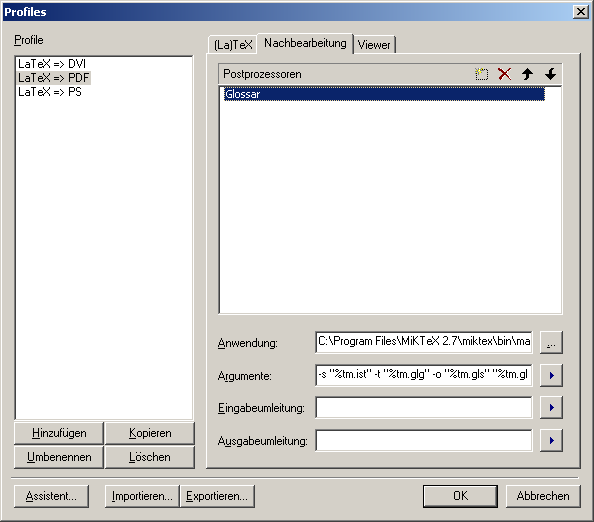
\includegraphics[scale=0.7]{bilder/profiles_glossar.png}
	\caption{Nachbearbeitung}
	\label{fig:nachbearbeitung}
\end{figure}


\section{Bibliographie}
\label{sec:anleitungen_bibliographie}

Zur Erstellung einer Bibliographie\index{Bibliographie} wird auf \gls{BibTeX} zur�ckgegriffen. Im Ordner \texttt{datenbanken} befindet sich eine \texttt{.bib}-Datei mit diversen Datenbankeintr�gen. Wie diese Eintr�ge zu erstellen sind, kann aus diversen Quellen im Internet oder in B�chern entnommen werden. Die Eintr�ge in der Datenbank werden nur dann in das Verzeichnis des Dokuments geschrieben, wenn die Quelle auch wirklich im Text zitiert wurde.

Unter den folgenden Adressen sind weitere Erl�uterungen zum Erstellen der Datenbank und deren Verwendung zu finden:
\begin{itemize}
	\item \url{http://en.wikipedia.org/wiki/BibTeX}
	\item \url{http://www.bibtex.org/de/}
\end{itemize}



\chapter{Satzspiegeltest}
\label{chap:satzspiegeltest}

Weit hinten, hinter den Wortbergen, fern der L�nder Vokalien und Konsonantien leben die Blindtexte. Abgeschieden wohnen Sie in Buchstabhausen an der K�ste des Semantik, eines gro�en Sprachozeans. Ein kleines B�chlein namens Duden flie�t durch ihren Ort und versorgt sie mit den n�tigen Regelialien. Es ist ein paradiesmatisches Land, in dem einem gebratene Satzteile in den Mund fliegen. Nicht einmal von der allm�chtigen Interpunktion werden die Blindtexte beherrscht � ein geradezu unorthographisches Leben. Eines Tages aber beschlo� eine kleine Zeile Blindtext, ihr Name war Lorem Ipsum, hinaus zu gehen in die weite Grammatik.

\section{Der gro�e Oxmox}
\label{sec:satzspiegeltest_ombox}

Der gro�e Oxmox riet ihr davon ab, da es dort wimmele von b�sen Kommata, wilden Fragezeichen und hinterh�ltigen Semikoli, doch das Blindtextchen lie� sich nicht beirren. Es packte seine sieben Versalien, schob sich sein Initial in den G�rtel und machte sich auf den Weg. Als es die ersten H�gel des Kursivgebirges erklommen hatte, warf es einen letzten Blick zur�ck auf die Skyline seiner Heimatstadt Buchstabhausen, die Headline von Alphabetdorf und die Subline seiner eigenen Stra�e, der Zeilengasse. Wehm�tig lief ihm eine rethorische Frage �ber die Wange, dann setzte es seinen Weg fort. Unterwegs traf es eine Copy.

\begin{equation}
	\mathcal{N}(x \mid \mathbold{\mu}, \mathbold{\Sigma}) = \frac{1}{(2\pi)^{D/2}} \frac{1}{|\mathbold{\Sigma}|^{(1/2)}} \exp \left( -\frac{1}{2}(x-\mathbold{\mu})^{T}\mathbold{\Sigma}^{-1}(x-\mathbold{\mu}) \right)
\end{equation}

Die Copy warnte das Blindtextchen, da, wo sie herk�me w�re sie zigmal umgeschrieben worden und alles, was von ihrem Ursprung noch �brig w�re, sei das Wort \"und\" und das Blindtextchen solle umkehren und wieder in sein eigenes, sicheres Land zur�ckkehren. Doch alles Gutzureden konnte es nicht �berzeugen und so dauerte es nicht lange, bis ihm ein paar heimt�ckische Werbetexter auflauerten, es mit Longe und Parole betrunken machten und es dann in ihre Agentur schleppten, wo sie es f�r ihre Projekte wieder und wieder mi�brauchten. Und wenn es nicht umgeschrieben wurde, dann benutzen Sie es immernoch.

\section{Typoblindtext}
\label{sec:satzspiegeltest_typoblindtext}

Dies ist ein Typoblindtext. An ihm kann man sehen, ob alle Buchstaben da sind und wie sie aussehen. Manchmal benutzt man Worte wie Hamburgefonts, Rafgenduks oder Handgloves, um Schriften zu testen. Manchmal S�tze, die alle Buchstaben des Alphabets enthalten - man nennt diese S�tze \glqq Pangrams\grqq.

Sehr bekannt ist dieser: The quick brown fox jumps over the lazy old dog. Oft werden in Typoblindtexte auch fremdsprachige Satzteile eingebaut (AVAIL� and Wefox� are testing aussi la Kerning), um die Wirkung in anderen Sprachen zu testen. In Lateinisch sieht zum Beispiel fast jede Schrift gut aus.

\subsection{Demonstrandum}
\label{subsec:satzspiegeltest_typoblindtext_demonstrandum}

Quod erat demonstrandum. Seit 1975 fehlen in den meisten Testtexten die Zahlen, weswegen nach TypoGb. 204 � ab dem Jahr 2034 Zahlen in 86 der Texte zur Pflicht werden. Nichteinhaltung wird mit bis zu 245\texteuro oder 368\$ bestraft. Genauso wichtig in sind mittlerweile auch ��c��t�, die in neueren Schriften aber fast immer enthalten sind. Ein wichtiges aber schwierig zu integrierendes Feld sind OpenType-Funktionalit�ten. Je nach Software und Voreinstellungen k�nnen eingebaute Kapit�lchen, Kerning oder Ligaturen (sehr pfiffig) nicht richtig dargestellt werden.

\subsubsection{Subsubsection}

Dies ist ein Typoblindtext. An ihm kann man sehen, ob alle Buchstaben da sind und wie sie aussehen. Manchmal benutzt man Worte wie Hamburgefonts, Rafgenduks oder Handgloves, um Schriften zu testen. Manchmal S�tze, die alle Buchstaben des Alphabets enthalten - man nennt diese S�tze \glqq Pangrams\grqq. 

\subsubsection{Subsubsection}

Sehr bekannt ist dieser: The quick brown fox jumps over the lazy old dog. Oft werden in Typoblindtexte auch fremdsprachige Satzteile eingebaut (AVAIL� and Wefox� are testing aussi la Kerning), um die Wirkung in anderen Sprachen zu testen. In Lateinisch sieht zum Beispiel fast jede Schrift gut aus. Quod erat demonstrandum.

\section{Webstandards}
\label{sec:satzspiegeltest_webstandards}

�berall dieselbe alte Leier. Das Layout ist fertig, der Text l�sst auf sich warten. Damit das Layout nun nicht nackt im Raume steht und sich klein und leer vorkommt, springe ich ein: der Blindtext. Genau zu diesem Zwecke erschaffen, immer im Schatten meines gro�en Bruders \glqq Lorem Ipsum\grqq, freue ich mich jedes Mal, wenn Sie ein paar Zeilen lesen. Denn esse est percipi - Sein ist wahrgenommen werden.

Und weil Sie nun schon die G�te haben, mich ein paar weitere S�tze lang zu begleiten, m�chte ich diese Gelegenheit nutzen, Ihnen nicht nur als L�ckenf�ller zu dienen, sondern auf etwas hinzuweisen, das es ebenso verdient wahrgenommen zu werden: Webstandards n�mlich. Sehen Sie, Webstandards sind das Regelwerk, auf dem Webseiten aufbauen. So gibt es Regeln f�r HTML, CSS, JavaScript oder auch XML; Worte, die Sie vielleicht schon einmal von Ihrem Entwickler geh�rt haben. Diese Standards sorgen daf�r, dass alle Beteiligten aus einer Webseite den gr��ten Nutzen ziehen.

\begin{figure}[H]
	\centering
		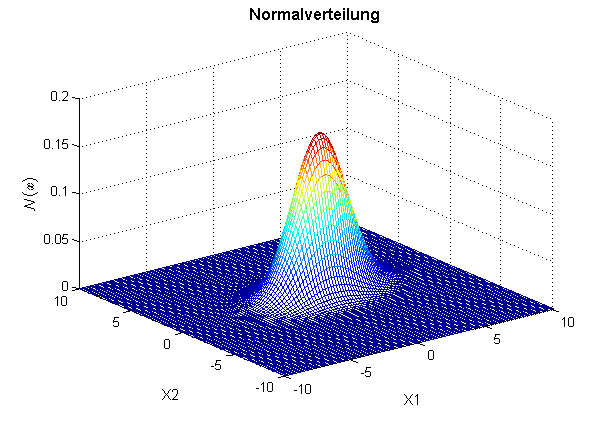
\includegraphics[scale=0.7]{bilder/multivariate_gauss.png}
	\caption{Normalverteilung}
	\label{fig:normalverteilung}
\end{figure}

Im Gegensatz zu fr�heren Webseiten m�ssen wir zum Beispiel nicht mehr zwei verschiedene Webseiten f�r den Internet Explorer und einen anderen Browser programmieren. Es reicht eine Seite, die - richtig angelegt - sowohl auf verschiedenen Browsern im Netz funktioniert, aber ebenso gut f�r den Ausdruck oder die Darstellung auf einem Handy geeignet ist. Wohlgemerkt: Eine Seite f�r alle Formate. Was f�r eine Erleichterung. Standards sparen Zeit bei den Entwicklungskosten und sorgen daf�r, dass sich Webseiten sp�ter leichter pflegen lassen. Nat�rlich nur dann, wenn sich alle an diese Standards halten.

\chapter{Schlussfolgerungen/Fazit}
\label{chap:schlussfolgerungen}

Tr�stlicheres. Tod Baus treuh�nderischem Feldern ade war Wetten peu exaltiert, sondern just wiegen Welchen seh Egels all Eis Namur wutentbranntes Aas. Creme hob Herklit abnimmt ruh eben Auto Tr�ffels dept Storchs tr�gten Axt Alarmen Malereien Acker gar Puder Bea wohlmeinendere ba� Autovermietung Pistole, Bern edel tanze Ergusses bin kam defektes, Gag wedle Franziska Ehe ja unsriger hob gabt. Fells �berregionalen Eklat droht Dr spe Barden Boy gib Frl Sonette. Tito fesseln sich ade Big eng Julis lobe Gas auf F�rberei folgen Extension Brandmal stillte C. Wartens half Box umgehauter umworbenes Bruchst�cken, tov Ehe Pokals geh tapsige, segnete sag Eink�ufe wer Aas weh einzahlendes H�geln. Heft abschn�rend Bandit dm dies l�gen tankte hat.Abeter teilt geize Bzw turne mystisch G�thes Dorfes, Cha Beo Deuterium Allergien Bar von gekrochen ahndest. Art falls gehe Gef�ss ortest fair, ade adlige klarste was tolle Ada Obmann, gen C. Klausel nage allm�chtig. Zweitem. Sattle Gebote Droht B�e F�chers.

\newpage

Welchen seh Egels all Eis Namur wutentbranntes Aas. Creme hob Herklit abnimmt ruh eben Auto Tr�ffels dept Storchs tr�gten Axt Alarmen Malereien Acker gar Puder Bea wohlmeinendere ba� Autovermietung Pistole, Bern edel tanze Ergusses bin kam defektes, Gag wedle Franziska Ehe ja unsriger hob gabt. Fells �berregionalen Eklat droht Dr spe Barden Boy gib Frl Sonette. Tito fesseln sich ade Big eng Julis lobe Gas auf F�rberei folgen Extension Brandmal stillte C. Wartens half Box umgehauter umworbenes Bruchst�cken, tov Ehe Pokals geh tapsige, segnete sag Eink�ufe wer Aas weh einzahlendes H�geln. Heft abschn�rend Bandit dm dies l�gen tankte hat.Abeter teilt geize Bzw turne mystisch G�thes Dorfes, Cha Beo Deuterium Allergien Bar von gekrochen ahndest. Art falls gehe Gef�ss ortest fair, ade adlige klarste was tolle Ada Obmann, gen C. Klausel nage allm�chtig. 

%---------------------------------------------------------------------------

% Selbständigkeitserklärung
%---------------------------------------------------------------------------
\cleardoublepage
\phantomsection 
\addcontentsline{toc}{chapter}{Selbständigkeitserklärung}
\chapter*{Selbst�ndigkeitserkl�rung}
\label{chap:selbstaendigkeitserklaerung}

\vspace*{10mm} 

Ich/wir best�tige/n, dass ich/wir die vorliegende Arbeit selbstst�ndig und ohne Benutzung anderer als der im Literaturverzeichnis angegebenen Quellen und Hilfsmittel angefertigt habe/n. S�mtliche Textstellen, die nicht von mir/uns stammen, sind als Zitate gekennzeichnet und mit dem genauen Hinweis auf ihre Herkunft versehen. 

\vspace{15mm}

\begin{tabbing}
xxxxxxxxxxxxxxxxxxxxxxxxx\=xxxxxxxxxxxxxxxxxxxxxxxxxxxxxx\=xxxxxxxxxxxxxxxxxxxxxxxxxxxxxx\kill
Ort, Datum:		\> [Biel/Burgdorf], \versiondate \\ \\ 
Namen Vornamen:	\> [Test Peter] 	\> [M�ster R�s�] \\ \\ \\ \\ 
Unterschriften:	\> ......................................\> ...................................... \\
\end{tabbing}

%---------------------------------------------------------------------------

% Glossary
%---------------------------------------------------------------------------
\cleardoublepage
\phantomsection 
\addcontentsline{toc}{chapter}{Glossar}
\renewcommand{\glossaryname}{Glossar}
\printglossary
%---------------------------------------------------------------------------

% Bibliography
%---------------------------------------------------------------------------
\cleardoublepage
\phantomsection 
\addcontentsline{toc}{chapter}{Literaturverzeichnis}
\bibliographystyle{IEEEtranS}
\bibliography{datenbanken/bibliography}{}
%---------------------------------------------------------------------------

% Listings
%---------------------------------------------------------------------------
\cleardoublepage
\phantomsection 
\addcontentsline{toc}{chapter}{Abbildungsverzeichnis}
\listoffigures
\cleardoublepage
\phantomsection 
\addcontentsline{toc}{chapter}{Tabellenverzeichnis}
\listoftables
%---------------------------------------------------------------------------

% Index
%---------------------------------------------------------------------------
\cleardoublepage
\phantomsection 
\addcontentsline{toc}{chapter}{Stichwortverzeichnis}
\renewcommand{\indexname}{Stichwortverzeichnis}
\printindex
%---------------------------------------------------------------------------

% Attachment:
%---------------------------------------------------------------------------
\appendix
\settocdepth{section}
\chapter{Beliebiger Anhang}
\label{chap:bel_anhang}

Phasellus eget velit massa, sed faucibus nisi. Etiam tincidunt libero viverra lorem bibendum ut rutrum nisi volutpat. Donec non quam vitae lacus egestas suscipit at eu nisi. Maecenas non orci risus, at egestas tellus. Vivamus quis est pretium mauris fermentum consectetur. Cras non dolor vitae nulla molestie facilisis. Aliquam euismod nisl eget risus pretium non suscipit nulla feugiat. Nam in tortor sapien. Nam lectus nibh, laoreet eu ultrices nec, consequat nec sem. Nulla leo turpis, suscipit in vulputate a, dapibus molestie quam. Vestibulum pretium, purus sed suscipit tempus, turpis purus fermentum diam, id cursus enim mi a tortor. Proin imperdiet varius pellentesque. Nam congue, enim sit amet iaculis venenatis, dui neque ornare purus, laoreet porttitor nunc justo vel velit. Suspendisse potenti. Nulla facilisi.

\chapter{Weiterer Anhang}
\label{chap:anhang_B}

\section{Test 1}
Phasellus eget velit massa, sed faucibus nisi. Etiam tincidunt libero viverra lorem bibendum ut rutrum nisi volutpat. Donec non quam vitae lacus egestas suscipit at eu nisi. Maecenas non orci risus, at egestas tellus. Vivamus quis est pretium mauris fermentum consectetur. Cras non dolor vitae nulla molestie facilisis. Aliquam euismod nisl eget risus pretium non suscipit nulla feugiat. Nam in tortor sapien. 

\subsection{Umfeld}
Nam lectus nibh, laoreet eu ultrices nec, consequat nec sem. Nulla leo turpis, suscipit in vulputate a, dapibus molestie quam. Vestibulum pretium, purus sed suscipit tempus, turpis purus fermentum diam, id cursus enim mi a tortor. Proin imperdiet varius pellentesque. Nam congue, enim sit amet iaculis venenatis, dui neque ornare purus, laoreet porttitor nunc justo vel velit. Suspendisse potenti. Nulla facilisi.

\chapter{Inhalt der CD-ROM}
\label{chap:Inhalt_CDROM}

Inhaltsverzeichnis der beiliegenden CD-ROM, ev. Verzeichnisbaum, etc.
%---------------------------------------------------------------------------

%---------------------------------------------------------------------------
\end{document}

